\chapter{Setting up the problem}

\section{The Data}

The data from which the training and testing datasets are generated comprise 27 3-dimensional grey scale images from CT scans stored as DICOM files. Each come accompanied by a 3D array of the same dimension indicating whether the corresponding voxel is in the Atrium (1) or not (0). These are stored in NRRD files, another popular file format for storing those things. Figure whatever shows an example of a slice in the transverse plane (x-y plane). 

\begin{figure}
\centering
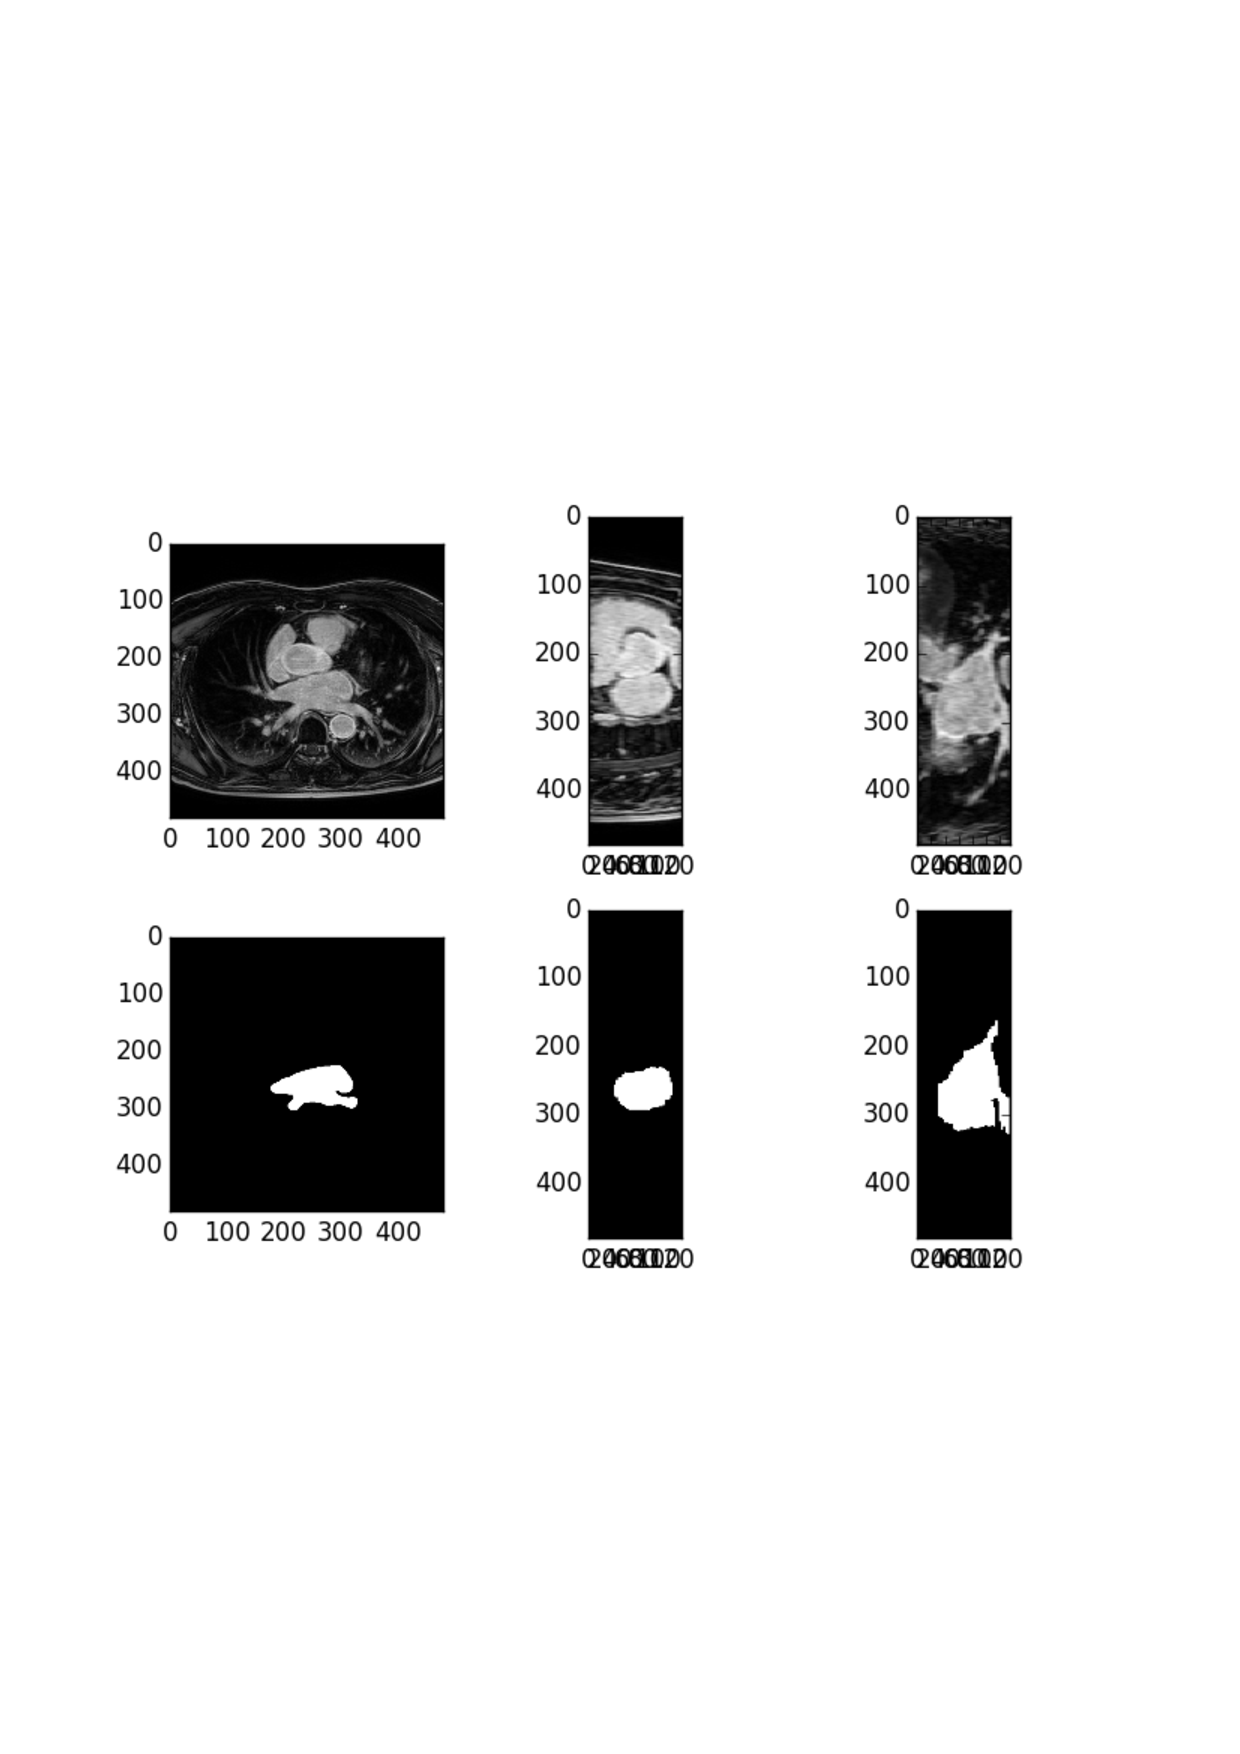
\includegraphics[trim=2cm 8cm 2cm 8cm, clip=true, height=80mm]{Chapter2/example_slice.pdf}
\caption{TODO include a example slice of a CT scan with the labelling for illustration purposes.}
\end{figure}

\section{The Tri-Planar Method}

Classifying the voxels require building an input set for each containing enough local and global information to allow the Neural Network to learn. A cheap way of doing so is to use the so-called tri-planar method [reference the paper that started it on knee cartilage]. This consists in generating 3 perpendicular square patches of dimension 32*32 in the transversal, saggital and coronal planes centred at the voxel of interest, thus providing 3 dimensional information while keeping the memory requirements low. In addition, we add 3 more compressed patches 5 times larger but resized to the same size to provide global information about the surroundings of concerned voxel. Each patch is then fed into a different input channel of the Convolutional Neural Network, and are then connected to the classifying layer using fully connected layers.

\section{Implementation Details}

\subsection{Libraries}

We use Torch, an open-source library maintained by Facebook in Lua, to train the Neural Networks and Python and a number of its libraries to handle all the logistics from generating the datasets to producing plots of segmentation results.

\subsection{Computer Power}

The code for training Neural Networks has been written to work on multi-GPU platforms as well as a single GPU to increase the speed of training many folds. The graphic cards consist in two NVIDIA Tesla K40m and two Tesla K20Xm.

